\documentclass[a4paper,14pt]{article}

%%% Работа с русским языком
\usepackage{cmap}					% поиск в PDF
\usepackage[T2A]{fontenc}			% кодировка
\usepackage[utf8]{inputenc}		% кодировка исходного текста
\usepackage[russian]{babel}	% локализация и переносы
%\usepackage[math]{pscyr}
%%% Дополнительная работа с математикой
\usepackage{amsmath,amsfonts,amssymb,amsthm,mathtools} % AMS
%% Номера формул
%\mathtoolsset{showonlyrefs=true} % Показывать номера только у тех формул, на которые есть \eqref{} в тексте.
%\usepackage{leqno} % Нумерация формул слева
%\usepackage{rumathgrk1}
%% Перенос знаков в формулах (по Львовскому)
\newcommand*{\hm}[1]{#1\nobreak\discretionary{}
	{\hbox{$\mathsurround=0pt #1$}}{}}
%%% Работа с картинками
\usepackage{graphicx}  % Для вставки рисунков
\graphicspath{{images/}{images2/}}  % папки с картинками
\usepackage{wrapfig} % Обтекание рисунков текстом

%%% Работа с таблицами
\usepackage{array,tabularx,tabulary} % Дополнительная работа с таблицами
\usepackage{longtable}  % Длинные таблицы
\usepackage{multirow} % Слияние строк в таблице
%%% Теоремы
\theoremstyle{plain} % Это стиль по умолчанию, его можно не переопределять.
\newtheorem{theorem}{Теорема}[section]
\newtheorem{proposition}[theorem]{Утверждение}

\theoremstyle{definition} % "Определение"
\newtheorem{corollary}{Следствие}[theorem]
\newtheorem{problem}{Задача}[section]

\theoremstyle{remark} % "Примечание"
\newtheorem*{nonum}{Решение}
%\pagestyle{empty}
%%% Страница
\usepackage{extsizes} % Возможность сделать 14-й шрифт
\usepackage{geometry} % Простой способ задавать поля
\geometry{top=20mm}
\geometry{bottom=35mm}
\geometry{left=30mm}
\geometry{right=20mm}
%


\usepackage{setspace} % Интерлиньяж
%\onehalfspacing % Интерлиньяж 1.5
%\doublespacing % Интерлиньяж 2
%\singlespacing % Интерлиньяж 1

\usepackage{lastpage} % Узнать, сколько всего страниц в документе.
\usepackage[usenames]{color}

\usepackage{bm}
\begin{document}
\textbf{Романов Андрей}

\textbf{Задание:}

\begin{figure}[h!]
	\centering
	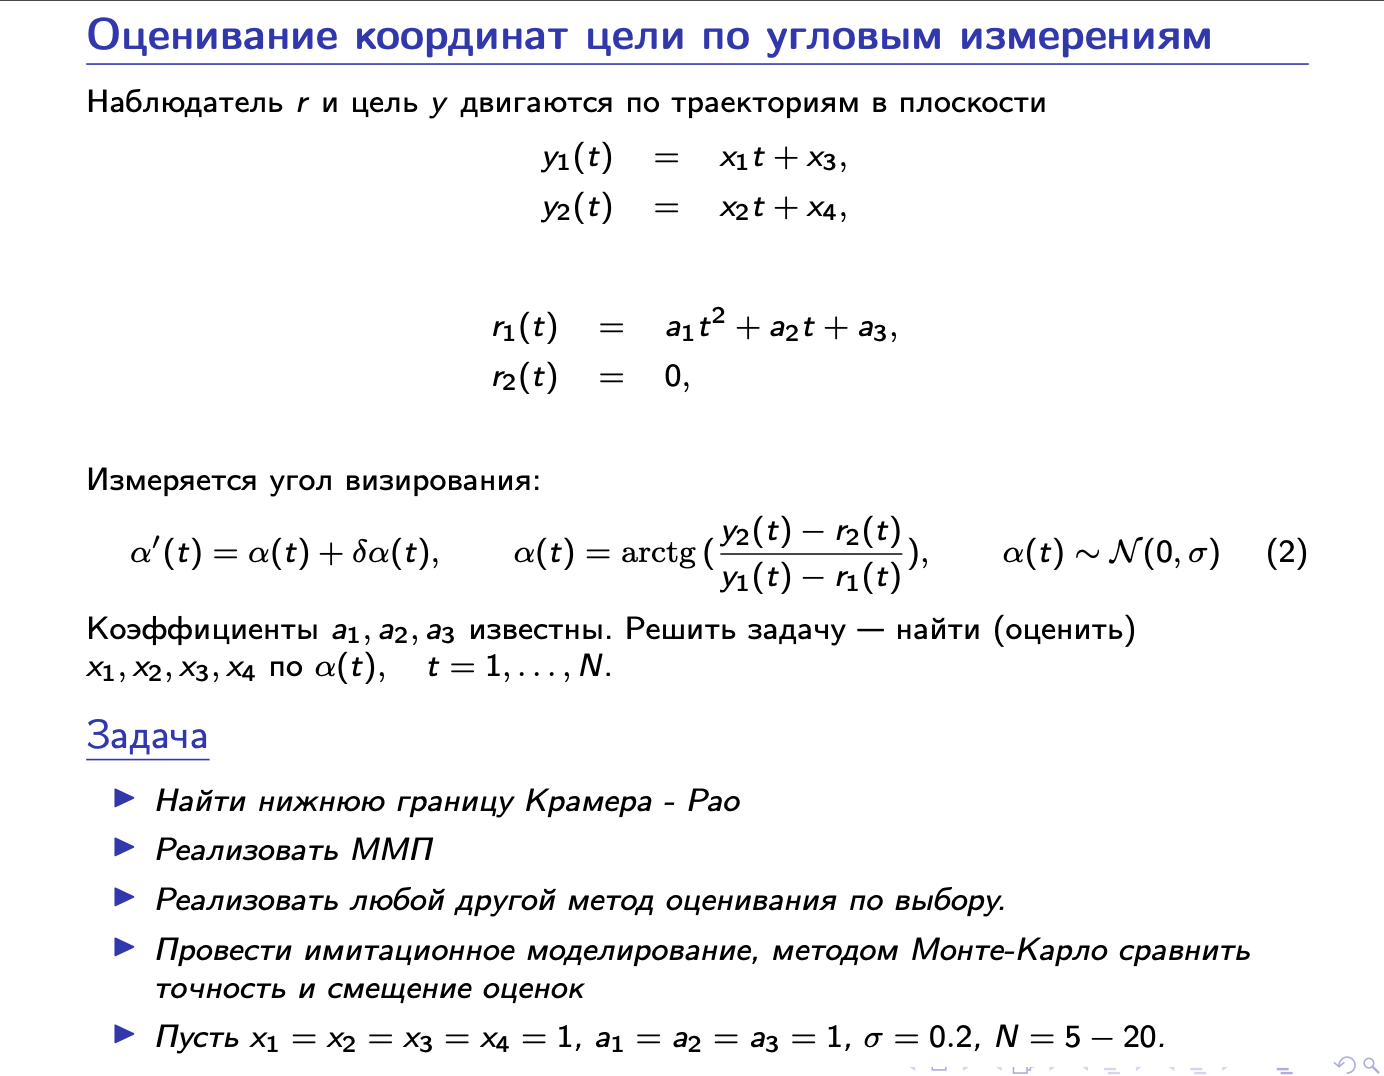
\includegraphics[width=0.9\linewidth]{tasks.png}
	\caption{Задание}
	\label{fig:gyrobus}
\end{figure}

\textbf{Решение:}

Для измерений
$y'=h(\Theta)+\delta y$

Матрица Крамера-Рао имеет вид
$\Phi(\theta)=\frac{\partial h}{\partial \theta}\cdot R^{-1} \cdot \left(\frac{\partial h}{\partial \theta}\right)^T$
$$\alpha'(t)=\arctan(\frac{x_1t+x_3-a_1t^2-a_2t-a_3}{x_2t+x_4})+\delta \alpha$$


Пусть 
$$B(t)=\frac{x_1t+x_3-a_1t^2-a_2t-a_3}{ x_2t+x_4}$$
$$
\frac{\partial h}{\partial x_1}=\frac{1}{1+B(t)^2}\cdot\frac{t(x_2+x_4)}{(x_2t+x_4)^2}=-\frac{1}{1+B(t)^2}\cdot\frac{t}{x_2t+x_4}
$$
$$
\frac{\partial h}{\partial x_2}=\frac{1}{1+B(t)^2}\cdot\frac{-t(x_1t+x3-a_1t^2-a_2t-a_3)}{(x_2t+x_4)^2}=\frac{1}{1+B(t)^2}\cdot\frac{-tB(t)}{x_2t+x_4}
$$
$$
\frac{\partial h}{\partial x_3}=\frac{1}{1+B(t)^2}\cdot\frac{x_2+x_4}{(x_2t+x_4)^2}=\frac{1}{1+B(t)^2}\cdot\frac{1}{x_2t+x_4}
$$
$$
\frac{\partial h}{\partial x_4}=\frac{1}{1+B(t)^2}\cdot\frac{-(x_1t+x3-a_1t^2-a_2t-a_3)}{(x_2t+x_4)^2}=\frac{1}{1+B(t)^2}\cdot\frac{-B(t)}{x_2t+x_4}
$$
\[
\Phi(x)=
\begin{pmatrix}
    \frac{\partial h_1}{x_1} & \frac{\partial h_2}{x_1}  & \dots & \frac{\partial h_N}{x_1} \\
    \frac{\partial h_1}{x_2} & \frac{\partial h_2}{x_2}  & \dots & \frac{\partial h_N}{x_2} \\
    \frac{\partial h_1}{x_3} & \frac{\partial h_2}{x_3}  & \dots & \frac{\partial h_N}{x_3} \\
    \frac{\partial h_1}{x_4} & \frac{\partial h_2}{x_4}  & \dots & \frac{\partial h_N}{x_4} 
\end{pmatrix}
\cdot
\begin{pmatrix}
    \frac{\partial h_1}{x_1} & \frac{\partial h_1}{x_2}  & \frac{\partial h_1}{x_3} & \frac{\partial h_1}{x_4} \\
    \frac{\partial h_2}{x_2} & \frac{\partial h_2}{x_2}  & \frac{\partial h_2}{x_3} & \frac{\partial h_2}{x_4} \\
    \hdotsfor{4} \\
    \frac{\partial h_N}{x_1} & \frac{\partial h_N}{x_2}  & \frac{\partial h_N}{x_3} & \frac{\partial h_N}{x_4} 
\end{pmatrix}
\cdot \frac{1}{\sigma^2}
\]
$$N=5;\sigma=0.2 =>D=8.47\cdot10^4$$
$$N=20;\sigma=0.2 =>D=9.94\cdot10^3$$
$$N=5;\sigma=0.02 =>D=847$$
$$N=20;\sigma=0.02 =>D=99$$
Для повышения точности изменим сделаем шаг времени $t=T/10$ и  $a2=-1$ тогда
$$N=20;\sigma=0.02 \Rightarrow D=0.59$$
$$N=100;\sigma=0.02 \Rightarrow D=0.0049$$

2) ММП

$$\alpha'=arctg(\frac{x_1t+x_3-a_1t^2-a_2t-a_3}{x_2t+x_4})+\delta \alpha$$

$$tg(\alpha'+\delta \alpha)=\frac{x_1t+x_3-a_1t^2-a_2t-a_3}{ x_2t+x_4}$$


$$
\frac{x_1t+x_3-a_1t^2-a_2t-a_3}{ x_2t+x_4}=tg \alpha'+\frac{\delta \alpha}{\cos^2\alpha'}
$$
$$
x_1t+x_3-a_1t^2-a_2t-a_3=tg \alpha'(x_2t+x_4)+\frac{\delta \alpha(x_2t+x_4)}{\cos^2\alpha'}
$$
$$
( x_1t+x_3-a_1t^2-a_2t-a_3-tg\alpha'( x_2t+x_4))\frac{\cos^2\alpha'}{t}=\delta \alpha(x_2+\frac{x_4}{t})
$$


\[ J=\sum_{t=1}^{N} \lVert( x_1t+x_3-a_1t^2-a_2t-a_3-tg\alpha'( x_2t+x_4))\frac{\cos^2\alpha'}{t} \rVert^2 \rightarrow \min \]
\[
A\cdot x=b
\]

\[
mult=\frac{\cos^2a'(t)}{t}
\]
\[
    mult\cdot
\begin{pmatrix}
    t_1 & -t_1\cdot \tg \alpha'(t_1)  & 1 & -tg \alpha'(t_1) \\
    t_2 & -t_2\cdot \tg \alpha'(t_2)  & 1 & -tg \alpha'(t_2) \\
    \dots & \dots & \dots & \dots \\
    t_N & -t_N\cdot \tg \alpha'(t_N)  & 1 & -tg \alpha'(t_N)
\end{pmatrix}
\cdot x =    mult\cdot
\begin{pmatrix}
    a_1t_1^2+a_2t_1+a_3 \\
    a_1t_2^2+a_2t_2+a_3 \\
    \dots  \\
    a_1t_N^2+a_2t_N+a_3 \\
\end{pmatrix}
\]
Далее применим МНК

3)
\end{document}